\section{Proposed Eco‐Driving GLOSA Algorithm}
\label{sec:Proposed_Eco_Driving_GLOSA_Algorithm}

This section presents the proposed eco-driving \ac{glosa} algorithm, which integrates real-time speed advisories with a fuel-aware optimization framework. The primary objective is to minimize the vehicle's total fuel consumption while ensuring it arrives at the stop line in synchrony with an upcoming green phase. This is achieved by combining three core components: (i) precise signal-timing prediction via the \ac{traci} interface, (ii) a two-phase kinematic trajectory model, and (iii) a detailed, emission-lookup-based cost functional. The online computation of the advisory speed is handled by the Python implementation communicating with \ac{sumo} via \ac{traci}.
\mynewline
The key components of the proposed method are as follows:
\begin{itemize}
    \item \textbf{Signal-Timing Prediction:} The controller leverages \ac{traci} functions to retrieve the current signal state and the time until the next phase transition. It iteratively scans the signal plan, considering multiple future cycles, to identify a feasible green window for the vehicle to target.

    \item \textbf{Kinematic Planning:} The vehicle's trajectory is modelled using a two-phase structure: an \emph{upstream} segment from its current position to the stop line, and a \emph{downstream} segment extending a fixed distance, \gls{ddown}, beyond the intersection. The algorithm optimizes a pair of constant accelerations, \gls{aup} for the upstream and \gls{adown} for the downstream segment, to find the most fuel-efficient path.

    \item \textbf{Emission-Lookup Cost Functional:} The cost function used for the optimization is designed to be highly accurate and flexible. Instead of relying on simplified coefficients, it computes the total fuel cost by integrating instantaneous fuel rates, $F(v,a)$, derived from detailed, pre-compiled lookup tables. This allows the framework to support multiple emission models, including the HBEFA4 polynomial model and the PHEMlight5 surface lookup, which were described in Section~\vref{subsubsec:detailed_emission_models}.
\end{itemize}

\subsection{Literature Foundation and Innovations}
\label{sec:EcoGlosa_Background}

The proposed eco-driving controller builds directly upon the eco-\ac{cacc}-Q framework introduced by Ala, Yang, and Rakha \cite{Ala2016}. Their work demonstrated that combining advisory speed control with an explicit model of queue dissipation can yield significant fuel savings on isolated approaches. The algorithm presented here preserves their fundamental two-phase trajectory structure, which consists of an upstream planning segment and a downstream recovery segment, but adapts and extends it for a real-time \ac{glosa} context.
\mynewline
This fundamental concept is depicted in Figure~\vref{fig:EcoGlosaConcept}'s conceptual time-distance diagram. The diagram uses several variables to label the trajectory segments and key events. Throughout this thesis, these correspond to the defined glossary symbols as follows: the upstream segment length, $d$, is denoted by \gls{dup}; the downstream segment length, $l$, by \gls{ddown}; and the initial queue length, $d_0$, by \gls{ells}. Similarly, the key time instances shown in the diagram correspond to the variables used in the controller's logic: the advisory start time, $t_0$, maps to \gls{tcur}, and the green signal onset, $t_g$, maps to \gls{tc}. As queue effects are not modelled in this study, the queue dissolution time, $t_c$, is assumed to be zero, making it coincident with the green onset, $t_g$.
\mynewline

\begin{figure}[htb]
    \centering
    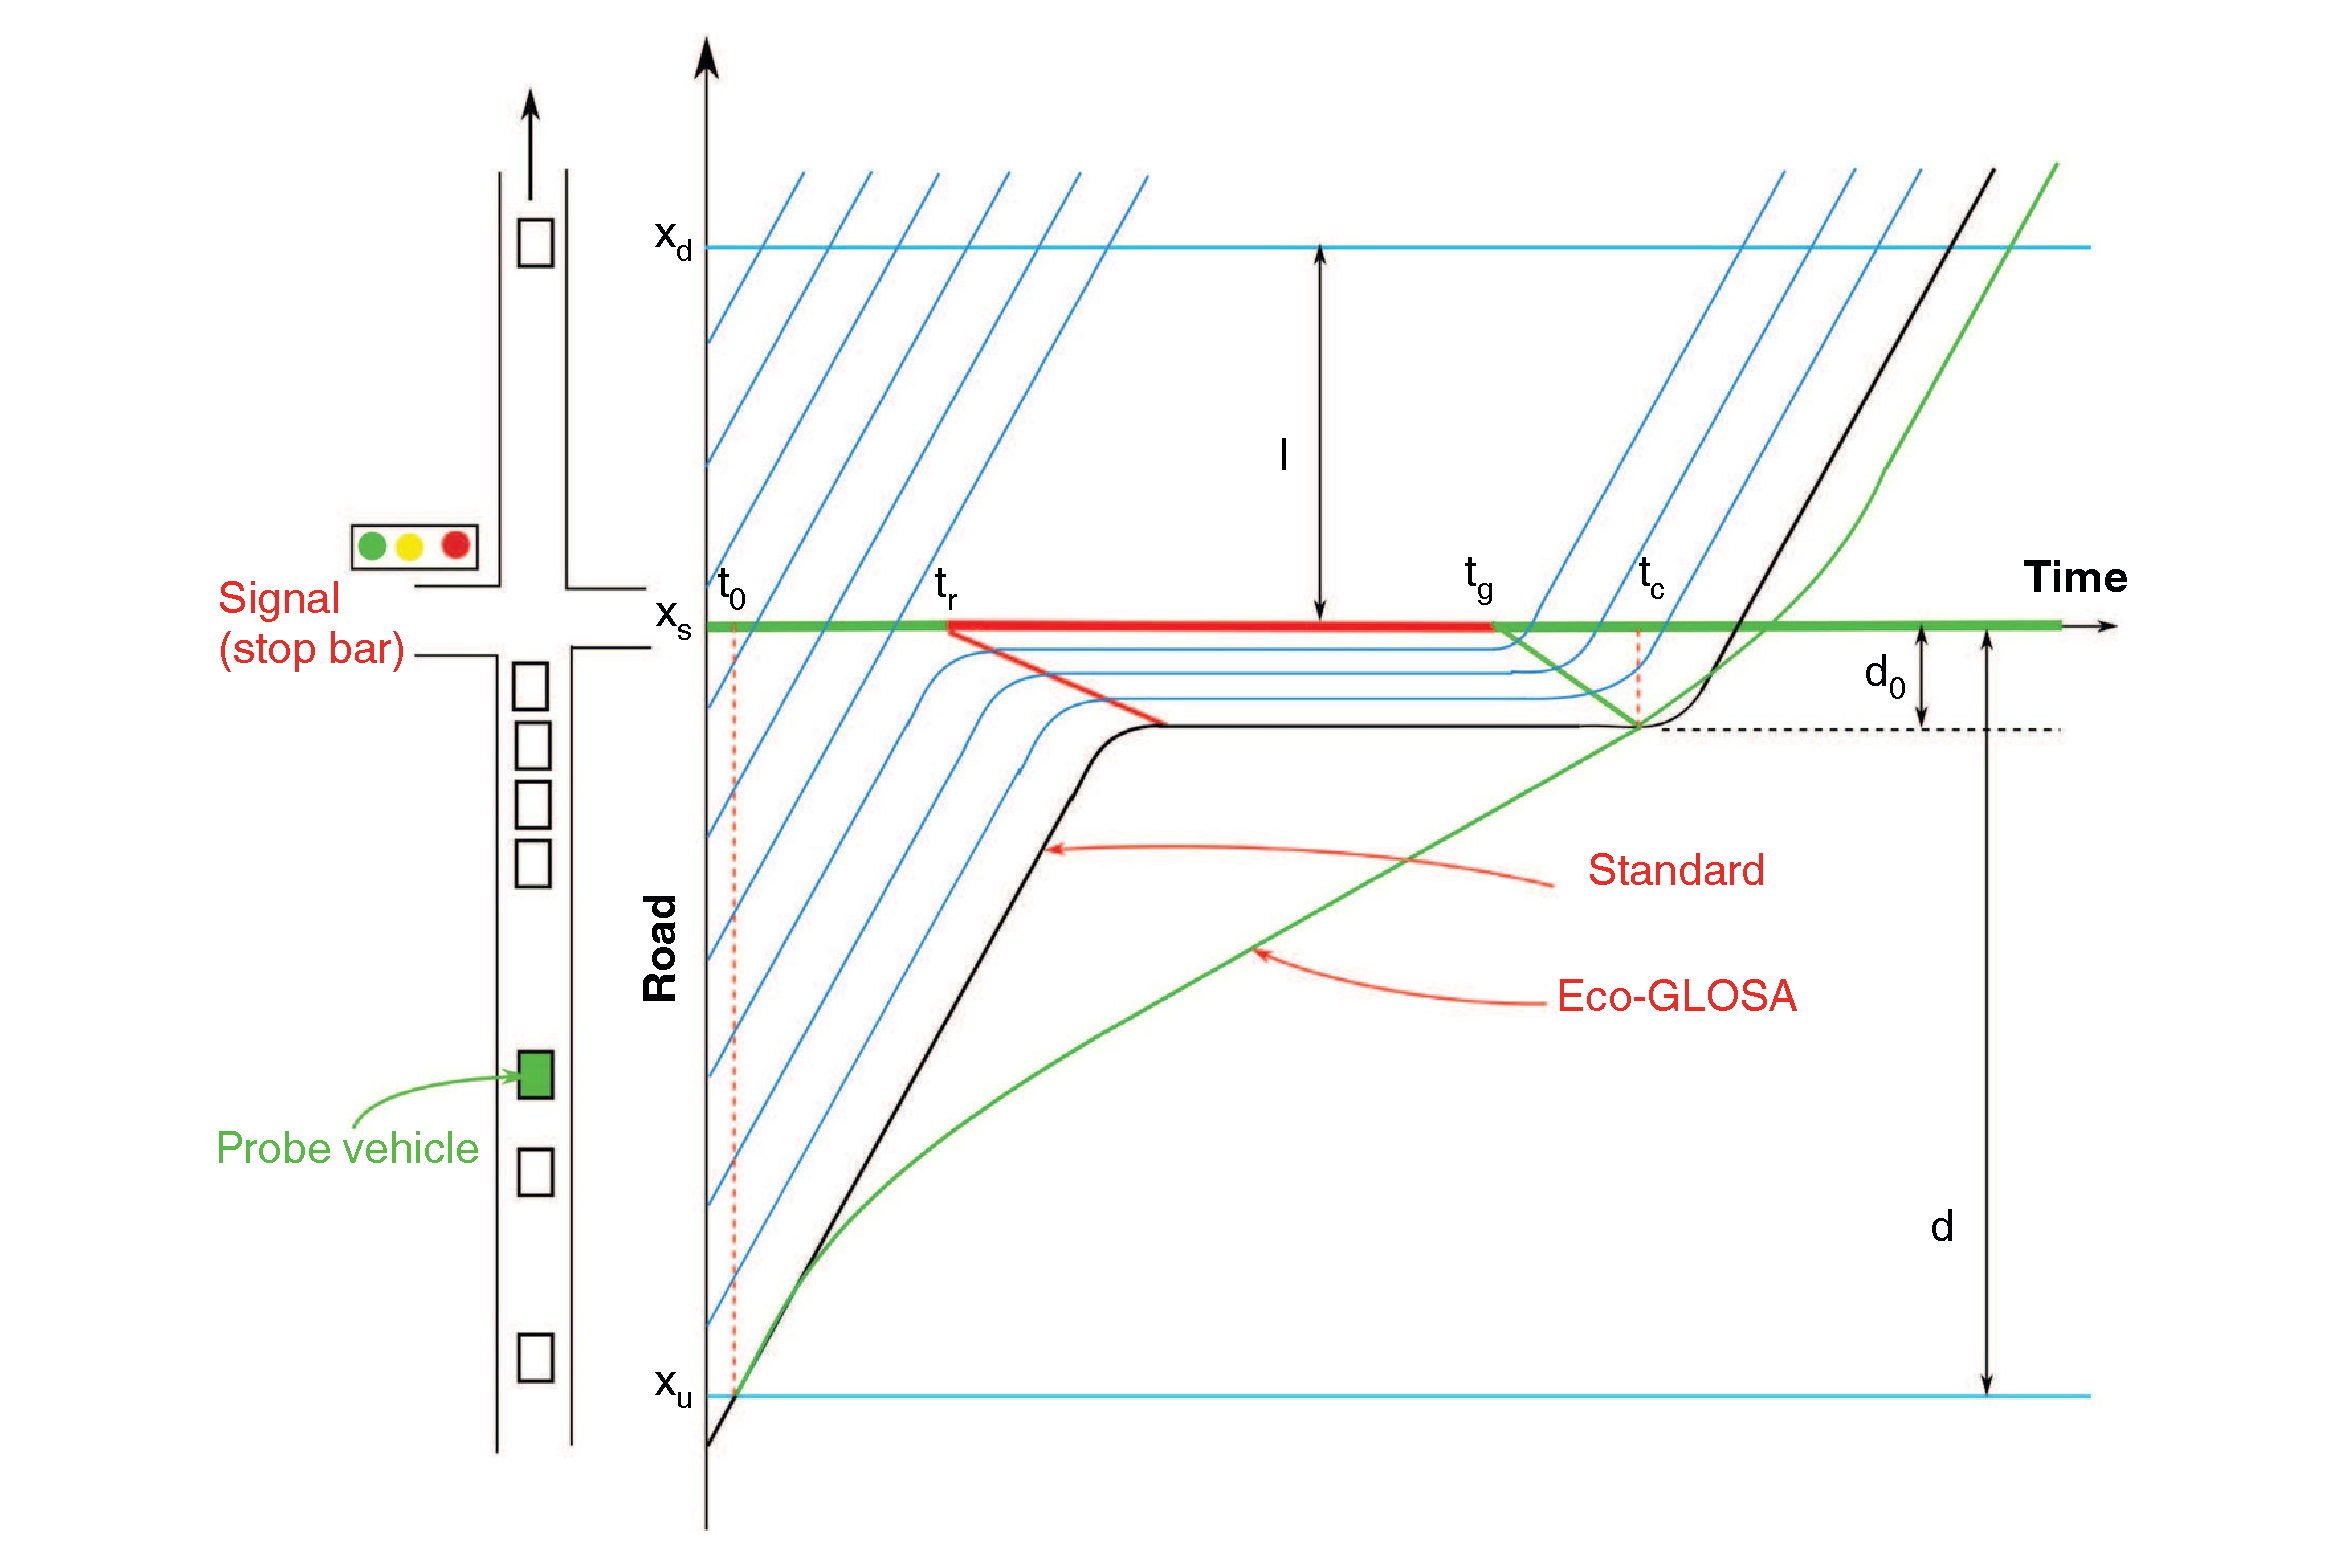
\includegraphics[width=0.9\textwidth]{data/img/GLOSA/ECO-GLOSA.pdf}
    \caption[Conceptual time-space diagram for the Eco-GLOSA algorithm]{%
        Conceptual time-space diagram of vehicle trajectories under standard control (dashed black line) and the proposed \ac{eco-glosa} (solid green line). The advisory is active between the starting point $x_u$ and the end point $x_d$. Key time instances include the start of the advisory ($t_0$), the onset of the red and green phases ($t_r$ and $t_g$), and the predicted queue dissolution time ($t_c$). \cite{Ala2016}
    }
    \label{fig:EcoGlosaConcept}
\end{figure}

The primary contributions of this work, which differentiate it from the foundational paper, are as follows:

\paragraph{Flexible Emission-Based Cost Function:} While the original work utilized VT-CPFM polynomial coefficients in its cost functional, this implementation replaces the single-model integrand with a flexible emission lookup module. This supports multiple high-fidelity models, including HBEFA4’s polynomial representation and PHEMlight5’s surface interpolation (as described in Section~\vref{subsubsec:detailed_emission_models}), allowing the optimizer to use more accurate, real-world data.

\paragraph{Expanded Two-Variable Optimization:} The optimization problem is extended to find the optimal pair of constant accelerations, $(\gls{aup}, \gls{adown})$, for the upstream and downstream segments, respectively. This is solved using a two-stage approach that combines a coarse brute-force grid search with a subsequent local hill-climbing refinement over the joint acceleration space. This contrasts with the original paper's focus on a single-variable refinement of the upstream acceleration only.

\paragraph{Real-Time \ac{glosa} Integration:} The entire optimization framework is embedded within a real-time \ac{glosa} context, using the \ac{traci} interface to receive live signal phasing and timing data from \ac{sumo}. This enables dynamic, multi-cycle phase scanning for online computation of the time-to-switch (\gls{tts}) and dynamic adjustment of the optimization horizon, eliminating the need for offline processing.

\paragraph{Practical Safety and Control Constraints:} Since the controller advises a \ac{sumo} vehicle rather than commanding direct acceleration inputs, several practical constraints are introduced. The algorithm's output is an advisory speed that is translated into a \gls{sf}, which is validated against permissible bounds $[\gls{minsf}, \gls{maxsf}]$. Furthermore, a minimum advisory speed, \gls{vmin}, is enforced post-optimization to ensure safe and realistic vehicle behaviour, a constraint not present in the original work.

While the foundational work by Ala et al. \cite{Ala2016} incorporated queue dissipation via shock-wave estimates, the experiments in this thesis disable explicit queue modelling to focus purely on the performance of the speed advisory component across different traffic densities. Collectively, these enhancements allow the proposed \ac{eco-glosa} algorithm to retain the methodological backbone of the original framework while achieving greater flexibility, realism, and fuel-efficiency in a real-time simulation setting.

\subsection{Algorithmic Framework}
\label{sec:EcoGlosa_Framework}

This part goes into detail about how the proposed eco-driving controller is structured and how its logic works. The overall workflow, from real-time data acquisition to the final speed advisory command, is conceptually illustrated in the flowchart in Figure~\vref{fig:EcoGlosa_Flowchart}. Building on the literature and innovations discussed previously, it first presents a high‐level overview of how the controller acquires environmental context and updates advisory speeds in each simulation step. Emphasis is placed on real‐time operation via the \ac{traci} interface, ensuring seamless integration of signal timing information, vehicle kinematics, and emission costs. The subsequent paragraphs describe the constructor’s static setup of vehicle and emission parameters, the per‐step invocation that locates the relevant traffic light and determines whether to issue speed advisories, and finally the core advisory routine that computes the optimal Speed Factor \gls{sf} or applies a fallback heuristic when necessary.

\begin{figure}[htb]
  \centering
  %–– Left half ––
  \begin{subfigure}[b]{0.49\textwidth}
    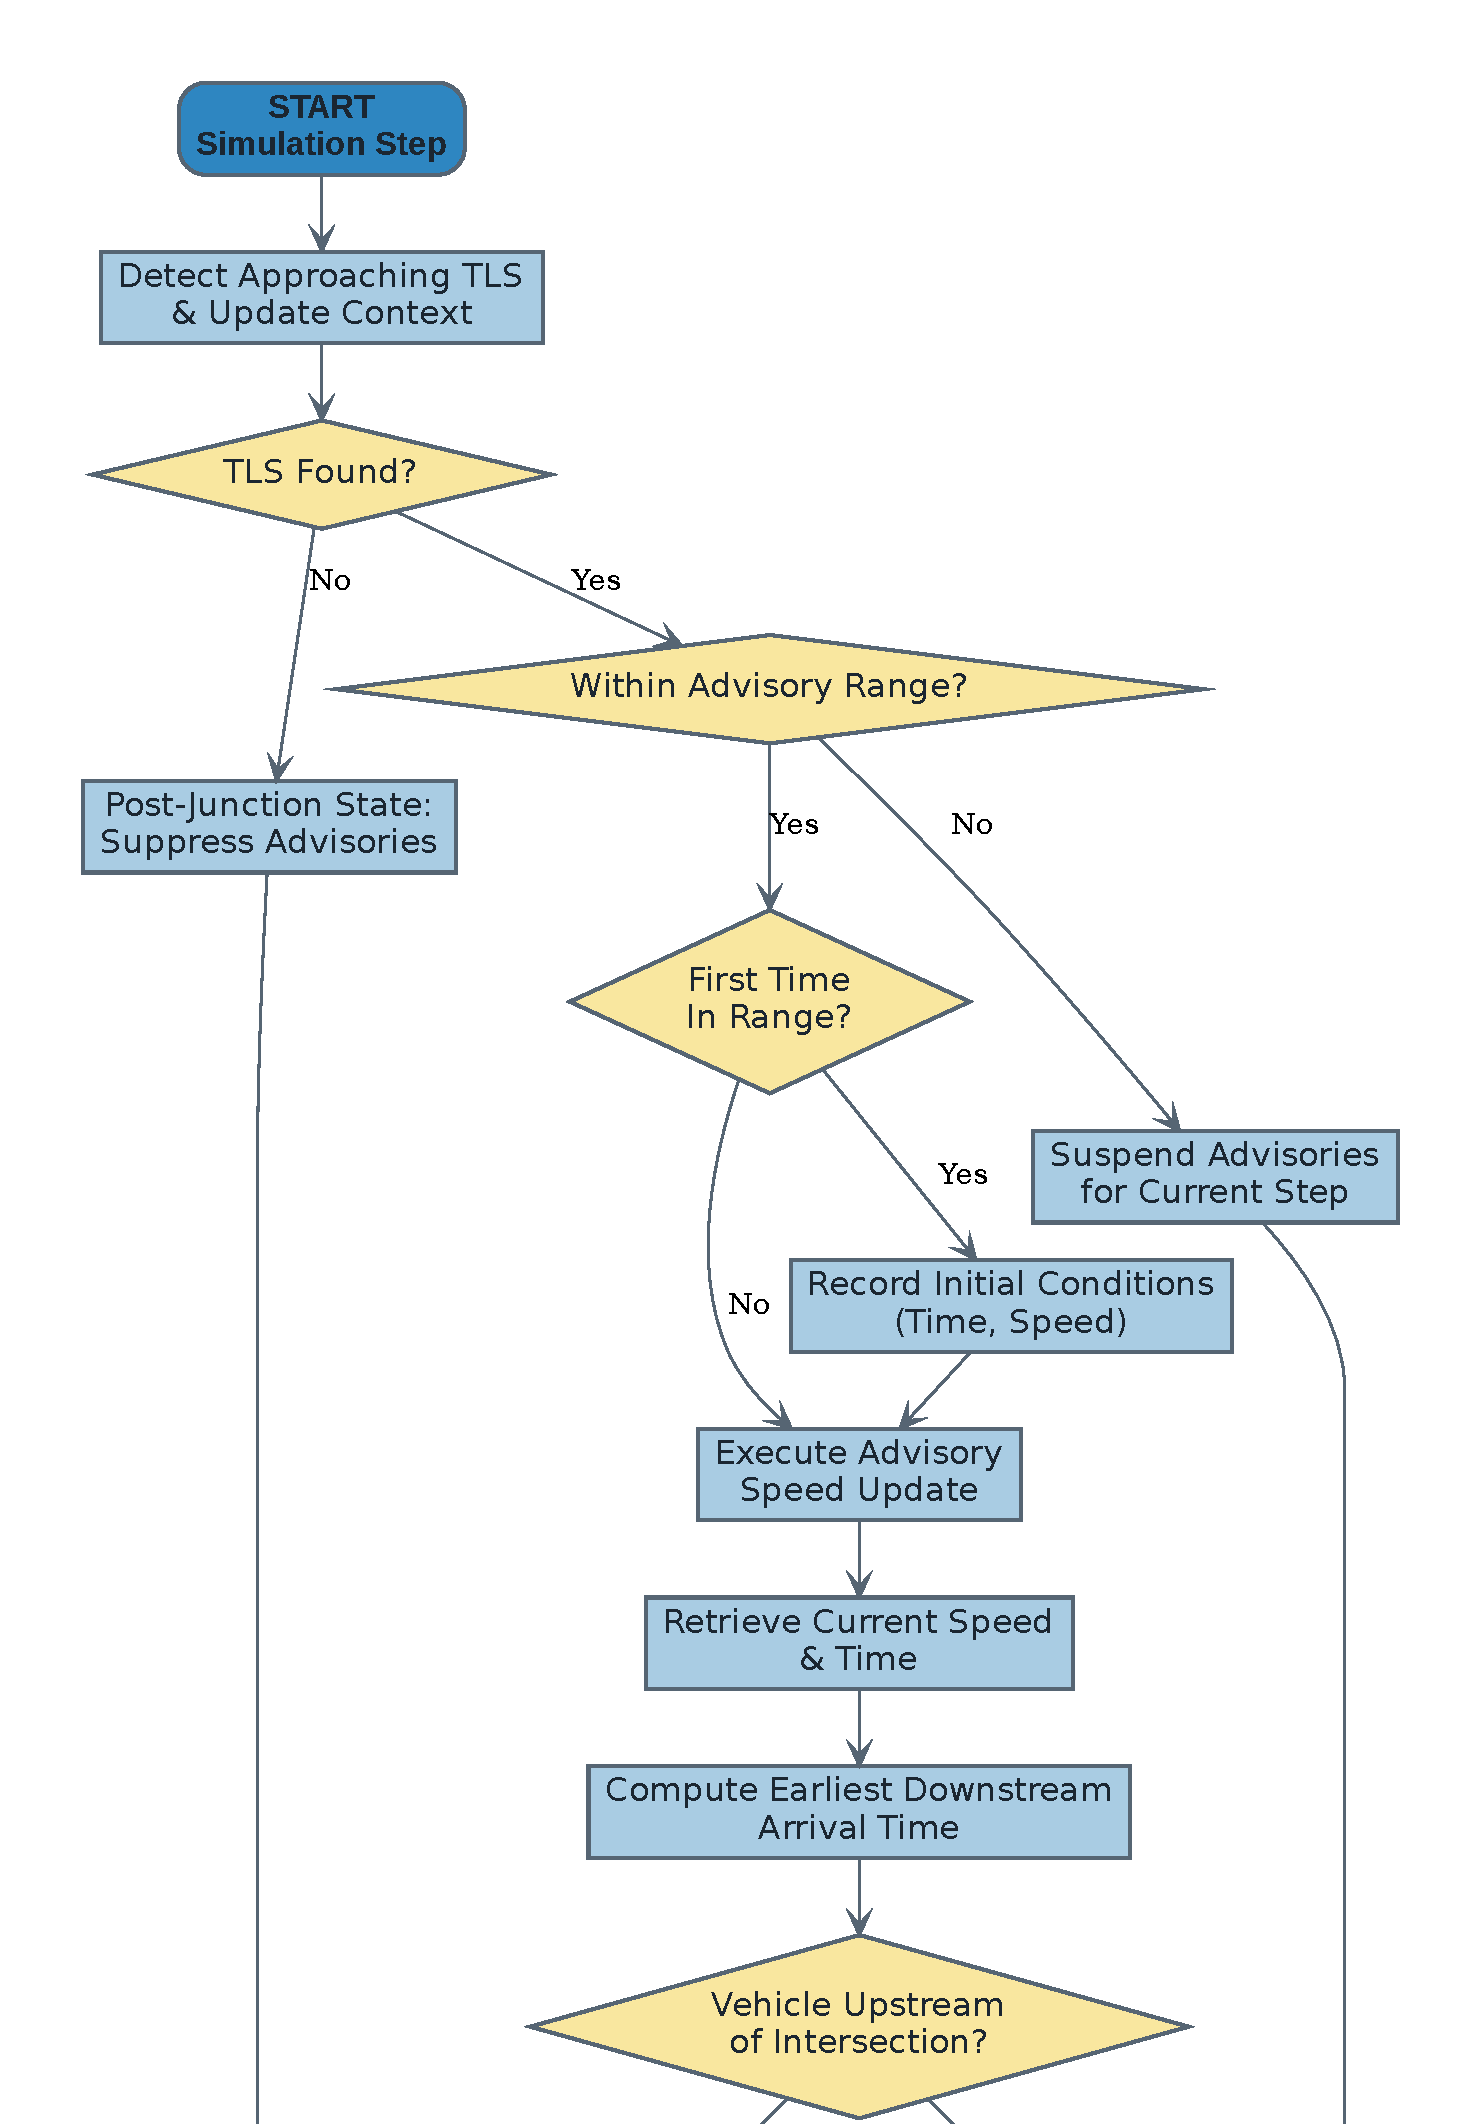
\includegraphics[
      page=1,
      width=\textwidth,
      keepaspectratio
    ]{data/img/GLOSA/glosa_flowchart_modern_simple.pdf}
    \caption{Initialization, TLS detection, and advisory preparation.}
    \label{fig:bigfig_part1}
  \end{subfigure}\hfill
  %–– Right half ––
  \begin{subfigure}[b]{0.49\textwidth}
    \includegraphics[
      page=2,
      width=\textwidth,
      keepaspectratio
    ]{data/img/GLOSA/glosa_flowchart_modern_simple.pdf}
    \caption{(Continued) Optimization, fallback, and advisory logic.}
    \label{fig:bigfig_part2}
  \end{subfigure}
  \caption[High-level flowchart of the \ac{eco-glosa} algorithm]{
    Full high-level flowchart of the proposed \ac{eco-glosa} controller’s logic. 
    Yellow diamonds represent decision points based on real-time simulation data, 
    blue rectangles denote computational or state-update actions, 
    and the red rectangle indicates the fallback heuristic triggered when the primary optimization fails.
  }
  \label{fig:EcoGlosa_Flowchart}
\end{figure}

\paragraph{Simulation‐Step Invocation and Junction Context Acquisition} 
\label{par:Simulation_Step_Invocation}

At each simulation time step, the controller checks if the vehicle is approaching a signalized intersection within a predefined advisory range. This is achieved by querying the simulation interface to identify the nearest upcoming signalized intersection and determine the vehicle’s current distance to it. If no relevant traffic light is detected, a post-junction state is assumed, and a residual downstream distance counter is updated. This prevents the generation of new advisories until the vehicle has fully cleared the previous junction and enters the control range of a new one. 
\mynewline
When a traffic light is detected and the vehicle enters the advisory range for the first time, the controller records the current time and vehicle speed as the initial conditions for the trajectory optimization. As long as the vehicle remains within the advisory range and upstream of the stop line, the speed advisory logic is continuously evaluated at each simulation step. Advisory generation ceases once the vehicle passes the intersection or exits the advisory range; it then remains inactive until the next relevant traffic light is encountered.

\paragraph{Advisory Speed Update Procedure}
\label{par:Advisory_Speed_Update_Procedure}
Upon the vehicle's entry into the predefined advisory range and prior to crossing the intersection, the controller initiates the main speed-update routine. This process begins by retrieving the current longitudinal speed, $\gls{vcur}$, and the current time, $\gls{tcur}$.
To determine the time required to cover the remaining distance to the lane's downstream limit, $\gls{ddown}$, under continuous maximum acceleration $\gls{amax}$ starting from $\gls{vcur}$, the controller solves the kinematic equation for time $t$:
\begin{equation}
   \gls{ddown} = \gls{vcur} \cdot t + \tfrac{1}{2} \gls{amax} \cdot t^2.
\end{equation}
The positive root of this equation, denoted as $\gls{tcontd}$, represents the duration required to cover $\gls{ddown}$ under continuous maximum acceleration. From this, the time required to accelerate to the allowed speed $\gls{vmax}$, if possible, is computed as:
\begin{equation}
    \Delta \gls{tacc}
    \;=\;
    \min\Bigl(\,\tfrac{\gls{vmax} - \gls{vcur}}{\gls{amax}},\;
    \gls{tcontd}\Bigr),
\end{equation}
where $\Delta \gls{tacc}$ denotes the duration of acceleration. The earliest feasible downstream arrival time, $\Delta \gls{tearliest}$, is then calculated by summing the acceleration time and the time required to cover the remaining distance at the maximum allowed speed, $\gls{vmax}$:
\begin{equation}
    \Delta \gls{tearliest}
    \;=\;
    \Delta \gls{tacc} \;+\;
    \frac{\gls{ddown} - \gls{dacc}}{\,\gls{vmax}\,},
\end{equation}
in which $\gls{dacc}$ is the distance covered during $\Delta \gls{tacc}$. The absolute end time of the downstream segment, $T_{\mathrm{end,down}}$, is defined by adding this earliest arrival time to the current simulation time:
\begin{equation}
    T_{\mathrm{end,down}} = \gls{tcur} + \Delta \gls{tearliest},
\end{equation}
where $T_{\mathrm{end,down}}$ represents the time at which the ego vehicle reaches the end of the downstream segment, i.e., the point beyond the intersection, based on the current simulation time and the earliest feasible arrival time.
\mynewline
Next, if the ego vehicle has not yet reached the intersection and remains in the upstream phase, the controller predicts the next feasible green onset. For each candidate traffic light phase, the controller evaluates if the estimated time-to-junction permits passage during the green interval:
\begin{equation}
   \gls{tttj} \;\le\; \Delta \gls{tswitch} + \gls{epsyellow},
\end{equation}
where $\gls{tttj}$ is the estimated time-to-junction, $\Delta \gls{tswitch}$ is the accumulated time until that phase switch, and $\gls{epsyellow}=0.5\,\unit{s}$ provides a safety buffer for yellow intervals. Once a suitable green onset is identified, the absolute time of this onset, $\gls{tc}$, is determined by adding the calculated duration from the current simulation time:
\begin{equation}
   \gls{tc}
   = \gls{tcur} + \Delta\gls{tswitch} + \gls{epsyellow}.
\end{equation}
The controller then determines the available slack time for optimization, which helps define a bounded yet adaptive time window for the trajectory planning:
\begin{equation}
   T_{\mathrm{slack,calc}} = \min\Bigl[\, \gls{tslack}\,(\gls{tenddown} - \gls{tcur}),\; \gls{tslackmax} \Bigr],
\end{equation}
where $\gls{tslack}=0.1\,\unit{s}$ is the base slack parameter and $\gls{tslackmax}=5\,\unit{s}$ specifies the maximum allowable slack time. This approach guarantees a bounded yet adaptive time window for optimization. 
\mynewline
To finalize the temporal bounds for optimization, the controller differentiates between two states of the ego vehicle: whether it is located downstream (i.e., having already crossed the stop line) or upstream (i.e., still approaching the intersection). If the ego vehicle is already in the downstream segment, the total end time for the optimization interval is computed as:
\begin{equation}
   T_{\mathrm{end}} = \gls{tenddown} + T_{\mathrm{slack,calc}},
\end{equation}
where $T_{\mathrm{end}}$ denotes the termination time of the optimization window. Conversely, if the vehicle remains upstream of the intersection, the end time is defined by:
\begin{equation}
   T_{\mathrm{end}} = \gls{tenddown} + T_{\mathrm{slack,calc}} + (\gls{tc} - \gls{tcur}),
\end{equation}
incorporating both the calculated slack time and the predicted duration to the green phase onset prior to intersection entry. This bifurcated approach ensures that the temporal optimization window is correctly adapted to the vehicle’s position with respect to the intersection, maintaining both feasibility and operational efficiency in the eco-driving control strategy.
\mynewline
Over the defined optimization horizon, the controller’s optimizer searches for the pair of constant accelerations, $(\gls{aup},\,\gls{adown})$, that minimizes the total fuel consumption and penalization cost, expressed by the following objective function:
\begin{equation}
\begin{aligned}
   \gls{Jcost} =\;
   &\underbrace{\int_{\gls{tcur}}^{\,\gls{tc}} F_{\mathrm{model}}\bigl(v(t),\,a(t)\bigr)\,dt}_{\text{upstream cost}}
   \;+\;
   \underbrace{\int_{\max(\gls{tcur},\,\gls{tc})}^{\,\gls{tend}} F_{\mathrm{model}}\bigl(v(t),\,a(t)\bigr)\,dt}_{\text{downstream cost}} \\
   &+\, \alpha_{\mathrm{speed}}\bigl(\gls{vmax} - v_{\mathrm{end}}\bigr)^2
   + \alpha_{\mathrm{time}}\bigl(t_{\mathrm{reach}} - T_{\text{down\_opt\_duration}}\bigr)^2,
\end{aligned}
\label{eq:costJ_highlevel}
\end{equation}
In this expression, $F_{\mathrm{model}}(v(t),\,a(t))$ denotes the instantaneous fuel consumption as a function of speed and acceleration. The first integral accumulates the upstream cost from the current time $\gls{tcur}$ to the predicted green phase onset $\gls{tc}$. The second integral accounts for the downstream cost, integrating from $\max(\gls{tcur}, \gls{tc})$ to the end of the optimization interval $\gls{tend}$. The penalty terms, weighted by $\gls{alphaspeed}$ and $\gls{alphatime}$, ensure that the terminal velocity $\gls{vend}$ remains close to the allowed cruising speed $\gls{vmax}$, and that the time at which $\gls{vmax}$ is reached, $\gls{treach}$, is close to the duration of the downstream optimization horizon, $T_{\text{down\_opt\_duration}}$, respectively. Here, $T_{\text{down\_opt\_duration}}$ is defined as $\gls{tend} - \max(\gls{tcur}, \gls{tc})$.
\mynewline
The optimization process employs a two‐stage procedure. \textit{Stage 1} involves sampling a uniform grid over
\begin{equation}
   \gls{aup},\;\gls{adown} \;\in\; \left[-\gls{amin},\,\gls{amax}\right],
\end{equation}
with a step size of $0.01$ to locate a coarse minimizer. \textit{Stage 2} then refines this solution by performing local hill‐climbing over the eight neighbouring acceleration pairs until no further reduction in $\gls{Jcost}$ is achieved. The optimizer returns the optimal accelerations, $\left(\gls{aup}^*,\,\gls{adown}^*\right)$, along with the corresponding advisory speeds $\gls{vc}$ and $\gls{vdown}$. Here, $\gls{vc}$ denotes the recommended speed for approaching the intersection, while $\gls{vdown}$ specifies the advisory speed to be maintained in the downstream segment after crossing the intersection. If $\gls{vc}$ falls below the minimum allowed speed $\gls{vmin}$, it is raised to $\gls{vmin}$ to preserve safety.
\mynewline
Should no feasible acceleration pair be found, an uncommon occurrence under light traffic but possible in dense conditions, the controller resorts to a fallback heuristic. This heuristic defines $\Delta T = \gls{tc} - \gls{tcur}$ and uses $\gls{dup}$ as the distance to be covered. While the theoretical acceleration required to cover distance $\gls{dup}$ within time $\Delta T$ starting from $\gls{vcur}$ can be derived from the kinematic equation as:
\begin{equation}
   \gls{dup} = \gls{vcur}\,\Delta T + \tfrac{1}{2}\,a_{\mathrm{up,fb}}\,(\Delta T)^2
   \quad\Longrightarrow\quad
   a_{\mathrm{up,fb}} = \frac{2\,\bigl(\gls{dup} - \gls{vcur}\,\Delta T\bigr)}{(\Delta T)^2},
\end{equation}
the controller's implementation simplifies this by choosing $a_{\mathrm{up,fb}}$ as either $\gls{amax}$ or $-\gls{amin}$ based on a calculated required speed. This selected $a_{\mathrm{up,fb}}$ is then used to determine a feasible single-segment trajectory. The resulting trajectory is re-evaluated for fuel cost (see \namevref{par:Emission_Model_BackEnd}), and its implied advisory speed is issued.
\mynewline
Finally, the optimal advisory speed factor is computed as follows:
\begin{equation}
\gls{sf} =
\begin{cases}
\dfrac{\gls{vc}}{\,\gls{vallowed}\,},
& \text{if } \gls{tcur} \leq \gls{tc}, \\[6pt]
\dfrac{\max\bigl(\gls{vdown},\,\gls{vmin}\bigr)}{\,\gls{vallowed}\,},
& \text{otherwise}.
\end{cases}
\end{equation}
\gls{sf} is subsequently applied to the ego vehicle within the simulation framework. Should the estimated arrival time at $\gls{vc}$ exceed the predicted green phase onset $\gls{tc}$ at any point, the controller re-evaluates and searches for a feasible green phase. This process continues until a valid solution is obtained, or the advisory horizon is exhausted.

\paragraph{Post‐Junction State Restoration}
Subsequent to the ego vehicle's navigation of the controlled segment, the controller ceases to issue active speed advisories, thereby allowing the resumption of the vehicle's default driving behaviour. The objective is to allow the restoration of original cruising parameters, such as the baseline speed factor, which ensures a seamless transition back to uninfluenced operation. Concurrently, the controller updates its internal state, marking the vehicle as being downstream of the intersection. This effectively suspends further advisory computations until a new relevant signalized junction is encountered on the vehicle's route.

\paragraph{Emission Model Back‐Ends}
\label{par:Emission_Model_BackEnd}
The controller integrates with two distinct fuel-rate back-ends, which are selectable at runtime through the emission database loaded during the initialization process. One option is the HBEFA4 polynomial model, which calculates instantaneous fuel consumption based on vehicle-specific emission class coefficients and fuel density. Alternatively, the PHEMLIGHT5 lookup model utilizes a two-dimensional grid of fuel consumption values, denoted by $FC(\gls{pkw},v)$, where $\gls{pkw}$ represents instantaneous engine power in kilowatts. The interpolated value from this grid undergoes corrections for vehicle mass and rated power, followed by conversion to the appropriate units. For both models, fuel consumption is set to zero if the engine is inactive for a period exceeding $10\unit{s}$ or if the vehicle is coasting ($a < \text{coast\_decel}(v)$). Both back-ends are consistently invoked within the cost integral of Equation~\vref{eq:costJ_highlevel} to compute accurate fuel consumption estimates for both upstream and downstream segments. A detailed explanation of these emission models is provided in Section \vref{subsubsec:detailed_emission_models}.